\section{Design for Manufacturing and Assembly}

Design for Assembly (DFA) is an engineering approach that focuses on designing products so that they can be assembled easily, quickly, and with fewer errors. The goal is to simplify the assembly process by reducing the number of parts, minimizing the need for special tools, and making components easy to handle and align. Some key principles of DFA include:

\begin{itemize}
    \item Minimising part count: Reducing the total number of components in a product can simplify assembly and reduce costs.
    \item Modularity: Similar products can be designed using common parts, which can simplify inventory management and assembly.
    \item Built-In Fasteners: Different types of fasteners, such as screws, rivets and bolts, should always be considered as a target for designing out. Although fasteners are rather inexpensive on their own, the installation process is really time-consuming.
    \item Use of standard parts: Reducing the amount of custom machining and fabrication made in-house and incorporating commercial off-the-shelf products into product design saves a lot of time and money. This includes motors, gears, springs, enclosures, etc.
\end{itemize}

\begin{figure}[H]
    \centering
    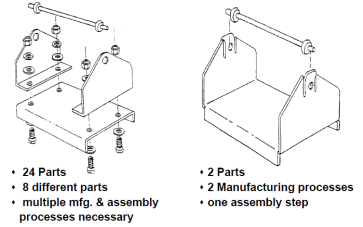
\includegraphics[width=0.6\textwidth]{theoretical-background/image/dfa_min_part_count.png}
    \caption{Minimising part count in Design for Assembly \cite{dfa_fractory}.}
    \label{fig:dfa_min_part_count}
\end{figure}

While DFA focuses on simplifying the assembly of parts, Design for Manufacturing (DFM) concentrates on making each part easier and more cost-effective to manufacture. Over 70\% of the product's final cost is determined during the design stage \cite{dfm_fractory}. Engineers are left with very little wiggle room for cost reduction once the design is settled. Usually, DFM is integrated in the early stages as this is the best time to conduct any redesigns. 

The combination of both DFA and DFM principles results in Design for Manufacturing and Assembly (DFMA), which aims to leverage the advantages of both these methodologies without the disadvantages of either.